%!TEX root = main.tex

\section{Design}
To achieve the two goals above, our design divided into three parts. First we design the ECN Interest sending rate on the receiver. Second we design a smart forwarding mechanism and at last we analysis the convergence and stability of the system.

\subsection{ECN Interest sending rate}
Our motivation is to send Interest at a maximum rate that the path can handle the corresponding coming back Data without dropping. To achieve this, every router on the path should calculates each flow's maximum Interest sending rate that it can handle, without causing congestion. We define such maximum rate as \emph{R(t)}.

Fig.\ref{fig-header}. shows the Interest and Data'ECN header. The ECN header contains the explicit congestion notification information on the path. The Interest carries the RTT of the flow. The RTT is defined as the interval between the receiver sends an Interest to the receiver receives the corresponding Data. In our design, RTT is used to determine the \emph{R(t)}'s updating interval. The provider copied the Interest's RTT to Data when it send back the Data, and the routers do not change it along the path. The router compares the \emph{R(t)} that is recorded in the Data with its own  \emph{R(t)}. If the router's rate is smaller, it replaces it. By this way, the coming back Data carries the minimum  \emph{R(t)} of all the routers along the path. As the Data comes back along the same path of the Interest, the rate on the Data also reflects the path of the Interest. Each receiver sends its Interest according the  \emph{R(t)} it receives from the Data.

\begin{figure}[t]
\centering
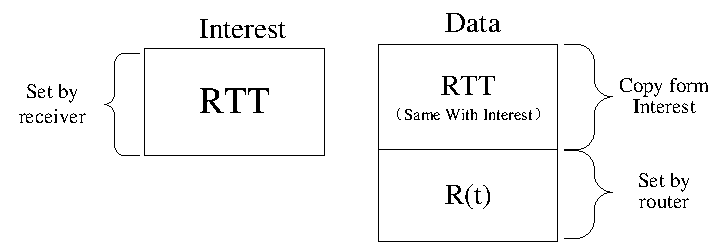
\includegraphics[width=3in]{header-ndn.pdf}
% where an .eps filename suffix will be assumed under latex,
% and a .pdf suffix will be assumed for pdflatex; or what has been declared
% via \DeclareGraphicsExtensions.
\centering
\caption{Explicit congestion notification header for Interest and Data.}
\label{fig-header}
\end{figure}
 Suppose we know how many flows going through a link, and we want to share its bandwidth with all the flows, then \emph{R(t)} can be calculated as follow:
\begin{equation}
R(t)=\frac{C}{Flow_{num}*Size_{d}}
\end{equation}

$\emph{Size}_{\emph{d}}$ is the size of incoming Data. $\emph{Flow}_{\emph{num}}$ is the flow number on the link. Eq. 1 is the ideal situation. When the network condition changes, such as the number of flows changes, \emph{R(t)} should update. To make the update reasonable and let the system enter stable situation, Eq. 1 should evolve as:
%\begin{small}
\begin{equation}
R(t)=R(t-RTT_{avg})+\frac{\alpha(C-S(t))-\beta\frac{Q(t)}{RTT_{avg}}}{Flow_{num}*Size_{d}}
\end{equation}
%\end{small}

\emph{R(t)} is the Interest sending rate that the router assigns to all flows at time \emph{t}. \emph{C} is the bandwidth of the link. \emph{S(t)} is the speed of coming back Data. \emph{Q(t)} is the packets that occupied in the queue at time t.  $\alpha$ and $\beta$ is the parameters that influence the convergence and performance.  $\emph{RTT}_{\emph{avg}}$ is the average RTT of all the flows that go through this router. We set $\emph{RTT}_{\emph{avg}}$ as \emph{R(t)}'s updating interval.

The reason we define the R(t) as Eq.2 is easy to understand. The available bandwidth and queue should be fairly share by all the flows, so the link's available resource is divided by the number of flow. If $\emph{(C-S(t))}>0$, there are more available bandwidth to be used and the rate should be increased. Otherwise, the bandwidth has been over used and the sending rate should be reduced. We assume that the packets occupied in the queue should always come to zero. If it is not zero, it means too many Datas flow into this link, and the Interest sending rate should be reduced. In every $\emph{RTT}_{\emph{avg}}$ the router should drain $\emph{Q(t)}/\emph{RTT}_{\emph{avg}}$ data. Because the R(t) is the Interest sending rate, and the available resource is supplied to the Data, so we divide it by the size of Data.

If the router want to make the system converse to stable stage more quickly, it can update the R(t) with shorter interval T $(0<T\leq\emph{RTT}_{\emph{avg}})$. Then  Eq. 2 becomes:
%\begin{small}
\begin{equation}
R(t)=R(t-T)+\frac{\frac{T}{RTT_{avg}}\ast(\alpha(C-S(t))-\beta\frac{Q(t)}{RTT_{avg}})}{Flow_{num}*Size_{d}}
\end{equation}
%\end{small}

Using the prefix of the Interest name to estimate how many flows go through the router will add complexity to the router. In\cite{RCP}, it has been proved that the processor-fair resource allocated way can estimate the flow number by the each flow's sending rate. Processor-fair means routers fairly give the link bandwidth and queue resource to all flows of this link. So we also use process-fair way to calculate how many flows go through this link:
%\begin{small}
\begin{equation}
Flow_{num}=\frac{C}{R(t-RTT_{avg})\ast{Size_{d}}}
\end{equation}
%\end{small}
As we set every flow share the link bandwidth equally, and every flow's rate is the same, it is reasonable to use Eq. 4 to estimate the number of flows. In Sec. \uppercase\expandafter{\romannumeral 5}, we will prove that the estimation is correctly.
Joining Eq.3 and Eq.4, Eq.3 becomes:
%\begin{scriptsize}
\begin{equation}
R(t)=R(t-T)[1+\frac{\frac{T}{RTT_{avg}}\ast(\alpha(C-S(t))-\beta\frac{Q(t)}{RTT_{avg}})}{C}]
\end{equation}
%\end{scriptsize}
Many factors may influence the size of Data in NDN, such as the different MTU of different link. So it will be very difficult to exactly measure the size of Data. When we need to use the size of Data to test the the accuracy of the flow number estimation, we have to use the historical information to estimate the size of Data. From Eq. 5 we can find that, R(t) do not need to measure the flow number directly and the size of Data. That will greatly simplify the router's calculating process.

Although our Interest sending rate's design principle is similar with RCP\cite{RCP}, our design process is different. In this paper we use \emph{R(t)} to control the receiver's sending rate, but RCP use the \emph{R(t)} to control the sender's packet sending rate. We also have to consider the size of Data, and in RCP the packet's size has not relationship with the design process.
\subsection{Smart adaptive forwarding}
In this paper we just control the forwarding process, not the route calculating process. The route algorithm in NDN is on active research, and it is still uncomplete. But from the algorithms proposed by now, we can see that the NDN route algorithm is different from TCP/IP\cite{ndnroute}. Traditional route protocol such as OSPF and RIP just have one single path for each destination. But in NDN, a data may be placed on different places, so there may be several paths to get a data. And even the data from the same provider may have different available paths. In this paper, we assume the receivers have several paths to get a data, and the routers have known every hop of different paths. The Smart adaptive forwarding mechanism we proposed just has relationship with the choose of forwarding interfaces from different paths.

Every router sends its own \emph{R(t)}, the transmit delay and the bandwidth of the next hop to the controller at an interval of $\emph{RTT}_{\emph{avg}}$. After several $\emph{RTT}_{\emph{avg}}$, the controller can know every router's \emph{R(t)} and the transmit delay of every hop. We call the information as forwarding-assistant information. The network's route information can also be stored in the controller. By the forwarding-assistant information and route information, we can calculate the best forwarding strategy. The forwarding-assistant and route information stored in the controller is showed in Fig.\ref{fig-assistant-information}.

\begin{figure}[t]
\centering
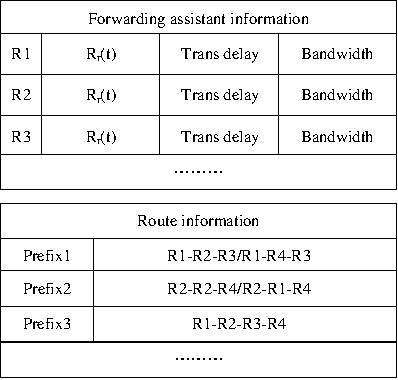
\includegraphics[width=2.5in]{forwarding-assistant-information.pdf}
% where an .eps filename suffix will be assumed under latex,
% and a .pdf suffix will be assumed for pdflatex; or what has been declared
% via \DeclareGraphicsExtensions.
\centering
\caption{Forwarding assistant and route information stored in the controller.}
\label{fig-assistant-information}
\end{figure}


Using the Interest sending rate we propose above, the FCT of each flow is:
%\begin{footnotesize}
\begin{equation}
FCT=\frac{Size_{f}}{Size_{d}\ast{R_{b}}}+RTT
\end{equation}
%\end{footnotesize}
$\emph{Size}_{\emph{f}}$ is the size of the flow. $R_{b}$ is the bottleneck's Interest sending rate. $R_{b}$ can be easily calculated by the forwarding-assistance and route information. Eq. 6 means that the FCT is the time that the flow goes through the bottleneck plus the RTT of this flow. The RTT of this flow can be calculated by the forwarding-assistant information.
We suppose flow i has serval available paths. If it chooses path j, then this flow's FCT on path j should be:
%\begin{footnotesize}
\begin{equation}
FCT_{i,j}=\frac{Size_{f}}{Size_{d}\ast{R^{'}_{b}}}+RTT_j
\end{equation}
%\end{footnotesize}
Where $RTT_j$ is the RTT of flow i if it chooses path j and $R^{'}_{bottleneck}$ is the bottleneck's Interest sending rate on path j.
%\begin{footnotesize}
\begin{equation}
R^{'}_{b}=\frac{C}{Flow_{num}+1}
=\frac{C}{C/(R_{b}\ast{Size_{d}})+1}
\end{equation}
%\end{footnotesize}
For simplify, we set the value of $Size_{d}$ and $Size_{f}$ as fixed values, and suppose $Size_{data} =Size_{flow}$. So Eq.7 becomes:
%\begin{footnotesize}
\begin{equation}
FCT_{i,j}=\frac{C/(R_{b}*Size_{d})+1}{C}+RTT_j
\end{equation}
%\end{footnotesize}
Our design goal is to minimum the Total Flow Complete Time (TFCT) in the network. TFCT is the sum of all the flows' complete time. To achieve our goal we define the objective of the smart forwarding as:
%\begin{footnotesize}
\begin{equation}\begin{aligned}
& \min &&  \sum_{i=0}^{n} FCT_i \\
& \text{s.t.}  && \text{path } j \text{ is available};\\
&              && \forall i, P_i \in \{0,1\};\\
&              && \max \min  R_i \enspace .
\end{aligned}
\end{equation}
%\end{footnotesize}
$P_i$ is the number of path that flow i chooses. $P_i \in \{0,1\}$ means $Flow_i$ can choose at most one path. $max \ min \ R_i$ means $Flow_{i}$'s Interest sending rate should be max . The reason we set $max \ min \ R_i$ is to achieve fairness between different flows.  If we do not set $max \ min \ R_i$, some flows may choose a min R to minimum the TFCT, and that will influence this flow's FCT. Sacrificing oneself to achieve the goal of minimum TFCT is unfair.

Routers send the updated forwarding-assistance and route information to the controller at the interval of $\emph{RTT}_{\emph{avg}}$. The routers send back smart forwarding decision for each flow when it receives the router's updating information. The smart forwarding decision is based on the unit of flow, not the unit of each packet. So the overhead introduced by the controller's help is very limited compared with the whole volume that goes through the router. To timely reflect the change of network information to the controller, routers can change the sending interval, and that will raise the overhead. But the balance between the overhead and the accuracy of updating information can be adaptively controlled.

\subsection{Stability analysis}
The parameters $\alpha$ and $\beta$ influence the stability and convergence of the system. As Eq. 2 shows, $\alpha$ influences how the bandwidth is use. If $\alpha$ is large then bandwidth will be occupied quickly. $\beta$ influences how quickly that the packets in the queue can be drained. Obviously that large $\alpha$ and $\beta$ can help the system to use the resource quickly. But large $\alpha$ and $\beta$ will make the system become unstable, as the network is difficult to convergence.

To choose suitable $\alpha$ and $\beta$ that make the system stable, we test under what $\alpha$ and $\beta$ , the flow number can be estimated accurately. Once the flow number of the network can be accurately estimated, the Interest sending rate \emph{R(t)} can also be estimated accurately, then the system will enter stable stage. So we choose the accuracy of estimating flow number as the stability evaluation criteria.

At first there are 10 flows in the network, and we test wether the flow number can accurately be estimated under different value of $\alpha$ and $\beta$ . Fig. \ref{fig-ab}. shows that under such values the flow number can be accurately estimated. Fig. \ref{fig-abwrong}. shows that under these values the estimated flow number change heavily which means that the system is not stable. From Fig. \ref{fig-ab}., we can find (0.2,1.5) is the most suitable value to estimate the flow number. Under this value, we test wether the system is still stable when the system changes. We set 5,10,15 and 20 flows in the network respectively. Fig. \ref{fig-abflownum}. shows that under different situation the flow number can also be accurately estimated when $\alpha=0.2 \beta=1.5$. That means a fit value of $\alpha$ and $\beta$ can make the system enter stable stage even when the system's situation changes.

From Fig. \ref{fig-abwrong}., we find that when $\alpha$ close to 0.5, the system becomes unstable, and when it is larger than 0.5, the system becomes even more unstable. We think it is because large $\alpha$ makes the system react too radically to increase \emph{R(t)}(when \emph{(C-S(t))}$>$0) or decrease \emph{R(t)}(when \emph{(C-S(t))}$<$0). Radical reaction will make the system difficult to converge. From Fig. \ref{fig-ab}., we find that when $\alpha$ $<$0.2, the system will take longer time to accurately estimate the flow number. It is because small $\alpha$ makes the system increase or decrease \emph{R(t)} conservatively, and that will result in longer time to convergence. When $\beta$ smaller than 1.5, although the system can be stable, the estimated flow number is not accurate compared with $\beta$ = 1.5. It is because small $\beta$ can not drain the packets in the queue quickly enough. And that will result in inaccurate \emph{R(t)} and flow number.

The key point of the stability analysis is that, for $\alpha$ and $\beta$ we can choose a fit value to make the system stable. Even when the system changes, such as the flow number, RTT and bandwidth, the fit value can also make the system keep stable. Although now we can not prove the best value by theory, it is possible to choose a suitable value by experimental test. In our simulation, we set $\alpha$ = 0.2 and $\beta$ =1.5, according the analysis above.
\begin{figure}[t]
\centering
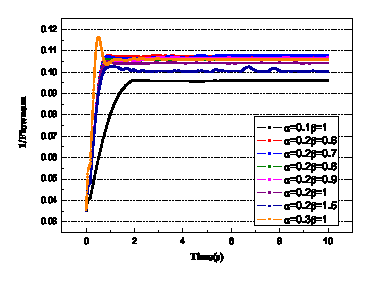
\includegraphics[width=2.5in]{ab-pic-cut.eps}
% where an .eps filename suffix will be assumed under latex,
% and a .pdf suffix will be assumed for pdflatex; or what has been declared
% via \DeclareGraphicsExtensions.
\centering
\caption{Under such $\alpha$ and $\beta$ the flow number can be accurately estimated.}
\label{fig-ab}
\end{figure}
\begin{figure}[t]
\centering
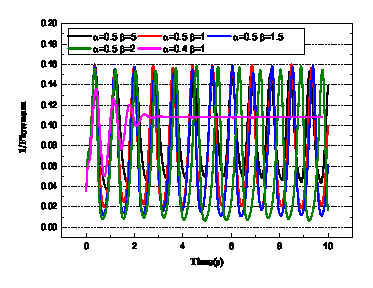
\includegraphics[width=2.5in]{abwrong-pic-cut.eps}
% where an .eps filename suffix will be assumed under latex,
% and a .pdf suffix will be assumed for pdflatex; or what has been declared
% via \DeclareGraphicsExtensions.
\centering
\caption{Under such $\alpha$ and $\beta$ the flow number can not be accurately estimated.}
\label{fig-abwrong}
\end{figure}
\begin{figure}[t]
\centering
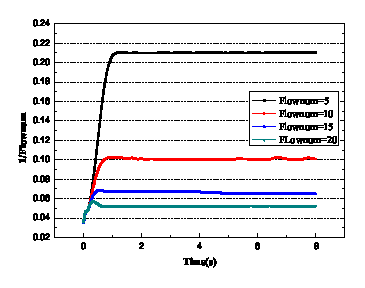
\includegraphics[width=2.5in]{abflownum-pic-cut.eps}
% where an .eps filename suffix will be assumed under latex,
% and a .pdf suffix will be assumed for pdflatex; or what has been declared
% via \DeclareGraphicsExtensions.
\centering
\caption{Stable $\alpha$ and $\beta$ can make the network stable even when network situation changes.}
\label{fig-abflownum}
\end{figure}

